\documentclass[11pt]{article}

\title{Dimensionality reduction \\ - \\ Concepts, and applications in scRNA-seq and DNA microscopy}
\author{Gergo Bohner}

\usepackage{graphicx}
\graphicspath{{fig/}}

\usepackage{hyperref}

\usepackage{amssymb}
\usepackage{amsmath}

\usepackage{tcolorbox} % Highlights text



% Defines

\DeclareMathOperator*{\argmin}{arg\,min}


\newcommand{\highlightbox}[1]{\colorbox{mysteelblue}{#1}}


\newcommand{\data}{\mathcal D}

\newcommand{\vecu}{\vec{u}}
\newcommand{\vecv}{\vec{v}}
\newcommand{\vecx}{\vec{x}}
\newcommand{\vecxbar}{\vec{\overline{x}}}
\newcommand{\vecy}{\vec{y}}
\newcommand{\vecyhat}{\vec{\hat{y}}}
\newcommand{\vecz}{\vec{z}}

\def\longhorz{\text{\vrule width3ex height.55ex depth-0.45ex}}
\def\longvert{\text{\vrule width.1ex height3ex depth0ex}}

\def\llongdash{\text{\vrule width6ex height.55ex depth-0.45ex}}
\def\llongvert{\text{\vrule width.1ex height6ex depth0ex}}

\def\lllongdash{\text{\vrule width9ex height.55ex depth-0.45ex}}
\def\lllongvert{\text{\vrule width.1ex height9ex depth0ex}}


\def\ldashcolvector#1{\begin{array}{c}\longvert\\#1\\ \longvert\end{array}}
\def\ldashrowvector#1{\longdash\; #1 \; \longdash}

\def\lldashcolvector#1{\begin{array}{c}\llongvert\\#1\\ \llongvert\end{array}}
\def\lldashrowvector#1{\llongdash\; #1 \; \llongdash}

\def\llldashcolvector#1{\begin{array}{c}\lllongvert\\#1\\ \lllongvert\end{array}}
\def\llldashrowvector#1{\lllongdash\; #1 \; \lllongdash}



\begin{document}

\maketitle

\tableofcontents


\section{The goals of dimensionality reduction}

Dimensionality reduction is a widely applied set of methods in various data analysis pipelines. It has three main aims:

\begin{itemize}
	\item \emph{Describe the data manifold} \\ Parametrise a space that we believe the observed data lives in. This space also serves as generalisation of where we expect future data to show up. Furthermore certain parameterisations  may facilitate interpretation of features.
	\item \emph{Reduce the observation noise} \\ We may separate the data variance into "within-manifold" (signal) and "out-of-manifold" (noise), this is called variance partitioning. Often only the within-manifold signal is used for further processing.
	\item \emph{Visualise the concepts discovered in the data} \\ Most collected data nowadays is very high (100+) dimensional, whereas most humans can only conceptualise a few dimensions at once. We have the responsibility to choose the most effective, yet accurate visualisations of the data to communicate features of the data - which may be even more informative together with information derived otherwise (such as derived clusters or external information).
\end{itemize} 



\subsection{Examples of specific goals}

Finding pure examples of specific dimensionality reduction applications is difficult, as dimensionality reduction methods are often used in conjunction with other techniques to communicate ideas. In the next few pages I show examples of well-defined, distinct applications of various dimensionality reduction methods, to help clarify the breadth of goals we may think of.
 
 \clearpage
 
\subsubsection{Manifold learning} 
(e.g. Isomap, LLE) \\ Estimate within-manifold distances, predict what data is likely in the future, learn about structure embedded within the data
 

\begin{figure}[h!]
\centering
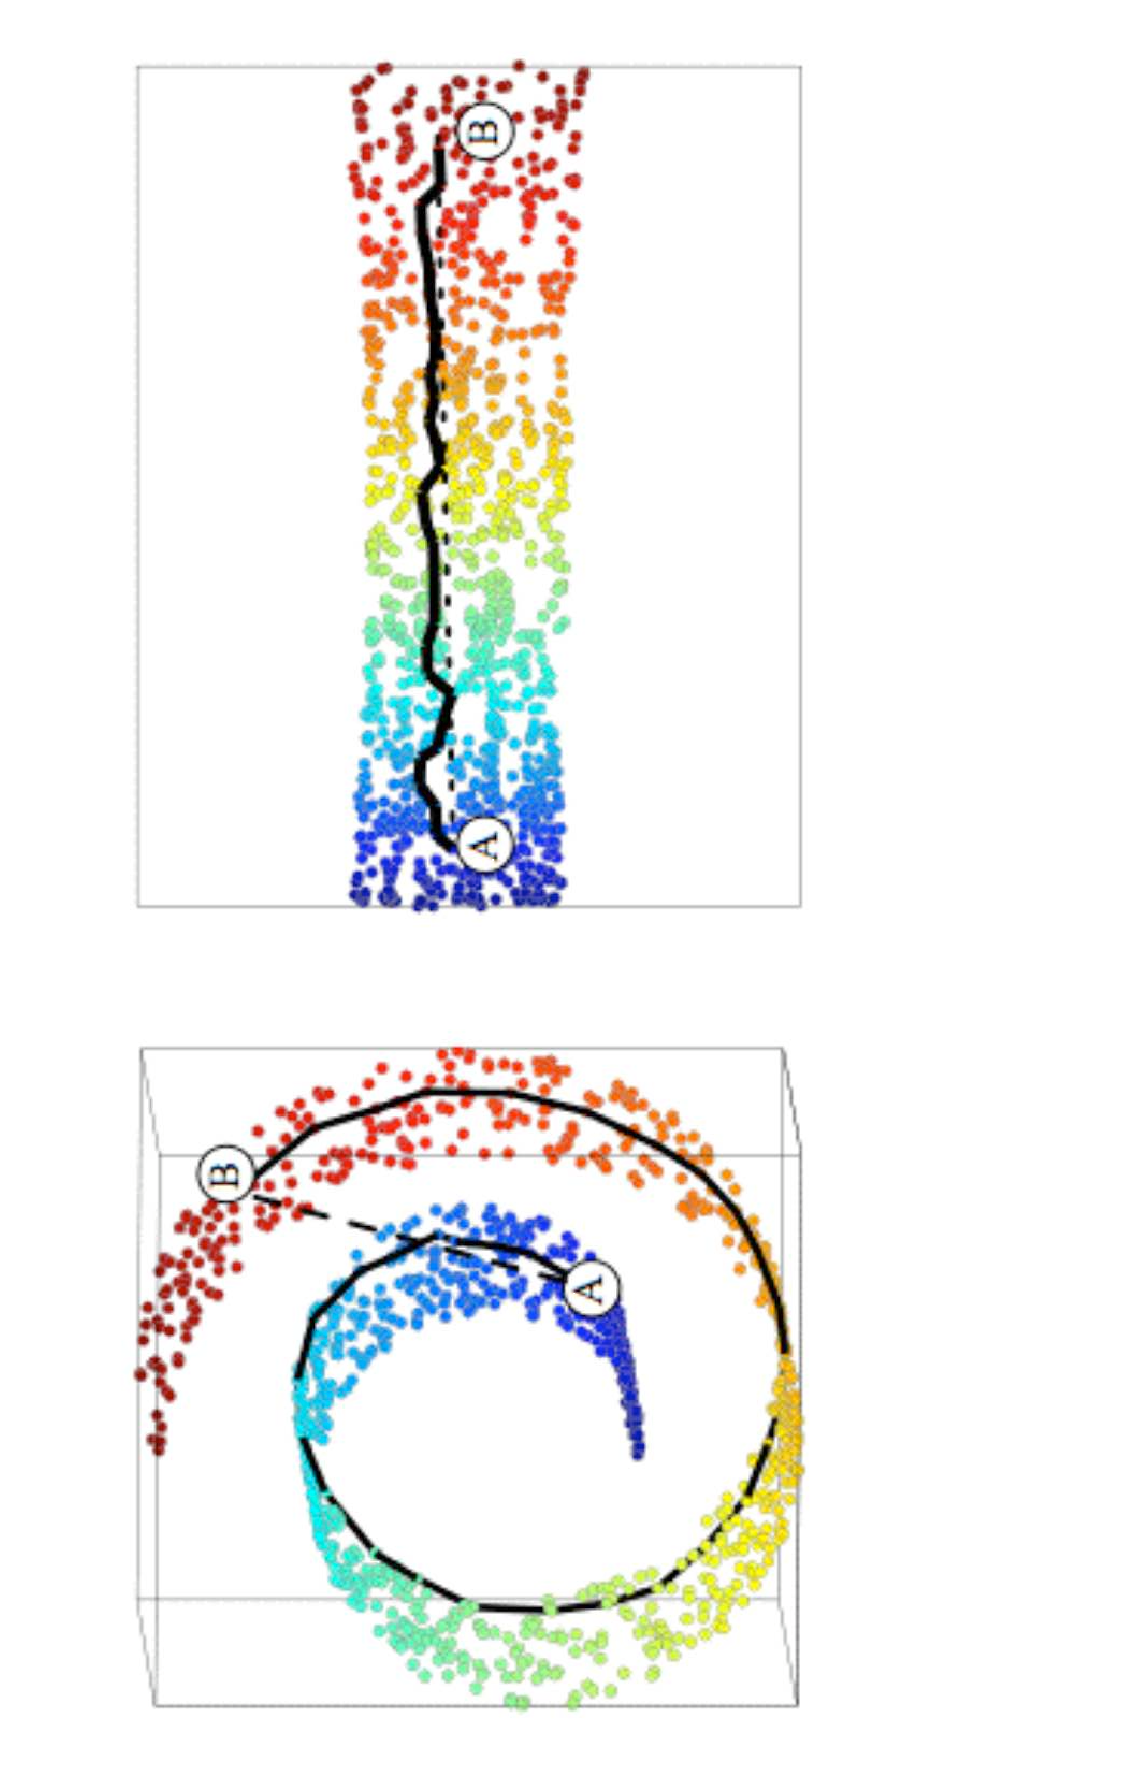
\includegraphics[width=0.73\textwidth]{swiss-unroll-distance}
\\ 
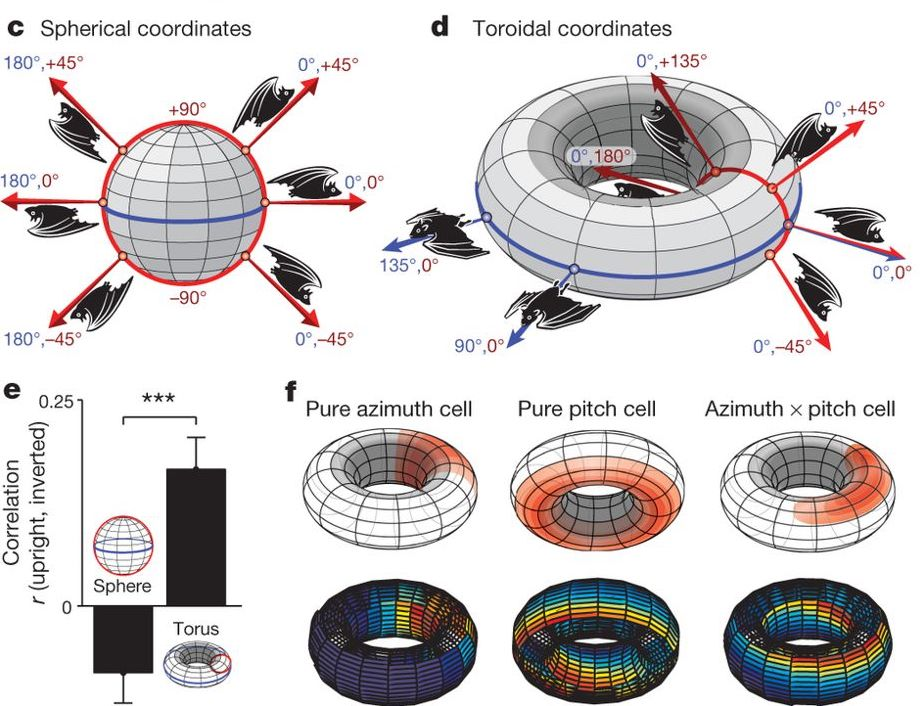
\includegraphics[width=0.5\linewidth]{bat_neurons_nature14031-f3} 
\caption{Examples for manifold estimation. (top) Swiss roll artificial dataset shows the concepts of a 2D manifold embedded in 3D (color purely serves as visual aid). (bottom) Comparing different manifold hypotheses (spherical vs toroidal) in behaving bats to explain neural variability \emph{(Finkelstein et al, Nature 2015)}}
\end{figure} 

\clearpage

 
\subsubsection{Feature discovery} 
(e.g. PCA, ICA, NMF) \\ Find a meaningful "basis" for the manifold - a set of features whose combination explains the data well, and leads to investigable hypotheses about the building blocks of the phenomenon that resulted in the collected data. 
 

\begin{figure}[h!]
\centering
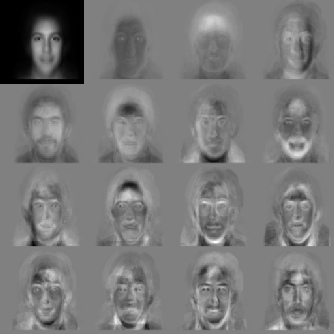
\includegraphics[width=0.5\linewidth]{eigfacessmall}
\caption{Example feature discovery - Given a corpus of grayscale face portraits, find the "average" face, and the main directions of variation (in pixel space). Note that even though the principal components are shown as 2D images, in reality the spatial structure is purely due to actual structure in the data, the algorithm was not looking for it (like convolutional neural nets explicitly do). }
\end{figure} 

\clearpage

 
\subsubsection{Reduce observation noise} (e.g. PCA, pPCA, FA, projection on manifold) \\ Experimenters can assume various sources of noise that is corrupting their input data, and select the appropriate method that is capable of separating signal from noise.
 

\begin{figure}[h!]
\centering
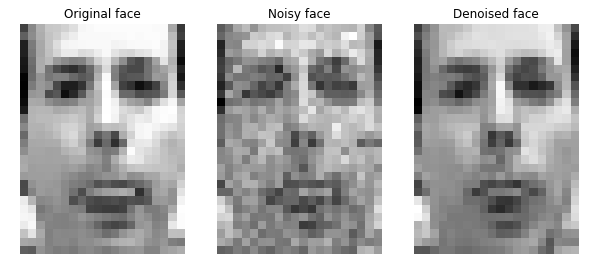
\includegraphics[width=0.75\linewidth]{pca_denoising_frey}
\\
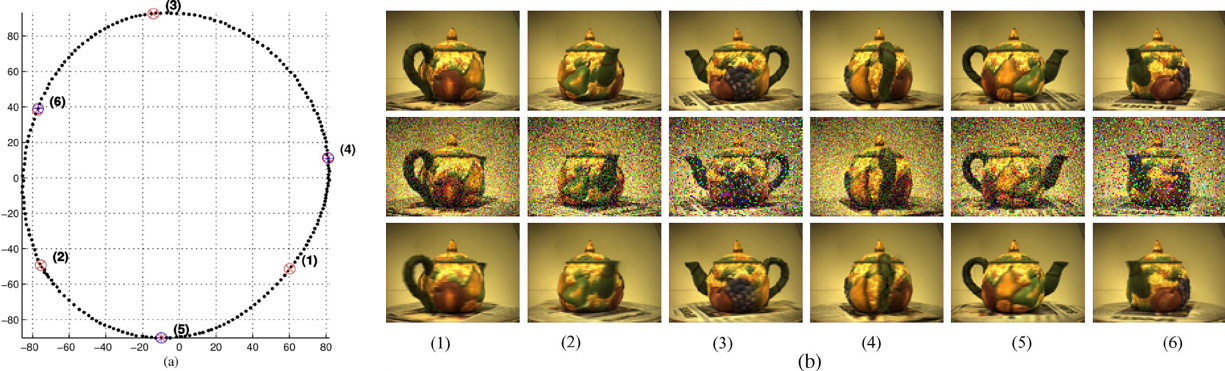
\includegraphics[width=1.0\linewidth]{nonlinear_denoising_teapot_cropped}
\caption{Denoising examples - (top) Using PCA to reduce the effects of additive, uniform and identically distributed Gaussian noise (PCA is optimal for this kind of noise). (bottom) Nonlinear manifold-based associative image denoising. Rotating teapot images embedded in low-D space (a), projection on learned manifold results in noise free images (b). \emph{Huang et al. Manifold-Based Learning and Synthesis} \url{doi 10.1109/TSMCB.2008.2007499}}
\end{figure} 

\clearpage

 
\subsubsection{Visualise high-D data via non-linear embedding} 
(e.g. LLE, Isomap, t-SNE) \\ Many dimensionality reduction methods have no easy-to-understand concepts in either a) what features of the high dimensional data they wish to keep unchanged in the low dimensional embedding or b) how they map from the high dimensional space to the low dimensional. \\ \\ Yet many of them become popular due to their ability to create embeddings in which humans may discover structure in, despite the lack of mathematical guarantees. These methods should be exclusively used for data visualisation, and to only communicate features or concepts of the data that have already been confirmed by other means (such as external information or clustering).
 

\begin{figure}[h!]
\hspace{-2cm}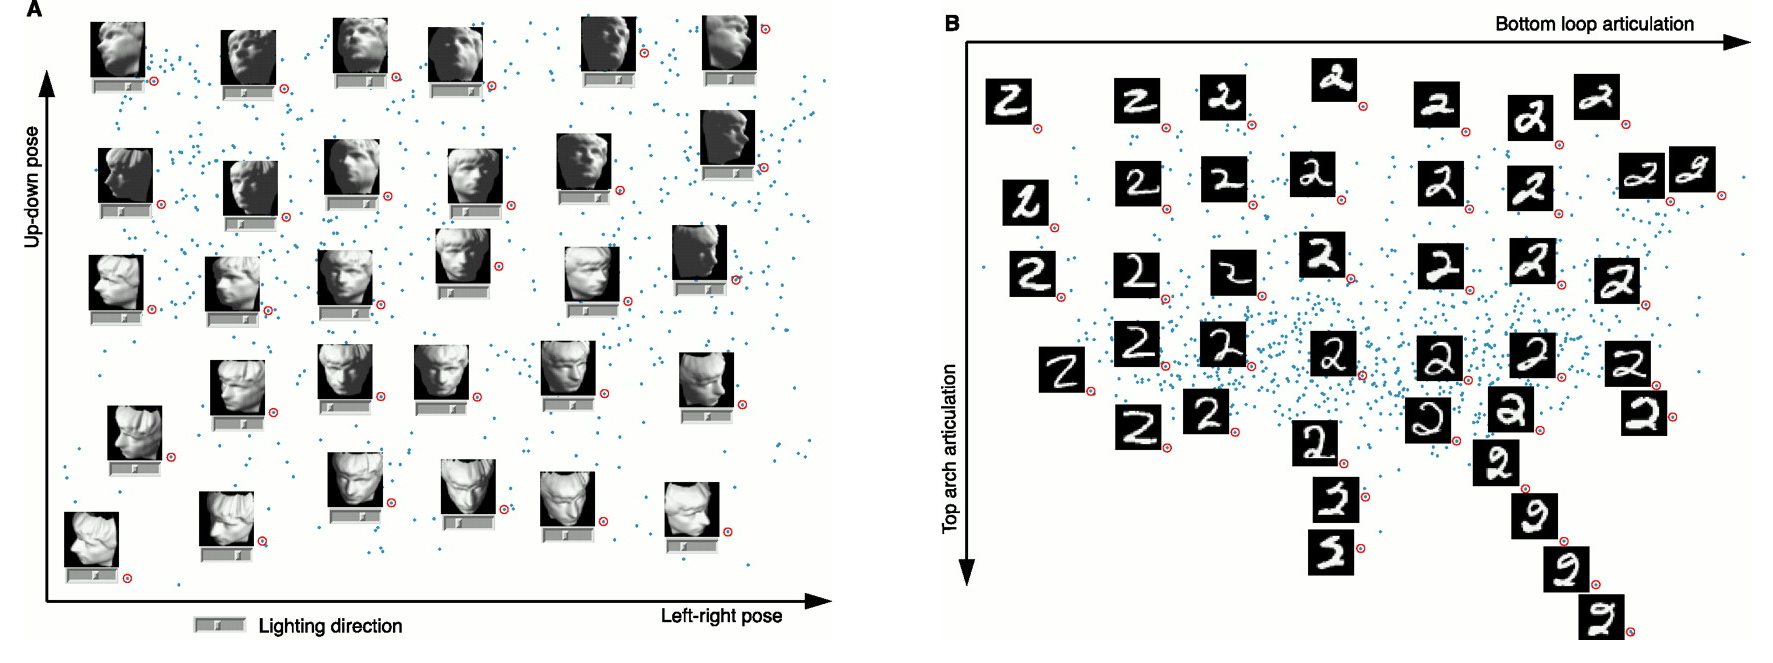
\includegraphics[width=1.3\linewidth]{isomap-head-digit-embeddings-2}

\caption{Visualising high-D data via isomap - Datasets can easily be projected into 3D (left) or 2D (right) spaces. Humans can then look at how samples change in the embedding space, and come up with interpretations for the axes. However, these interpretations then need to be treated as hypothesis, translated back into provable mathematical definitions, and shown to be supported by the data. \emph{J. B. Tenenbaum et al. ISOMAP - A Global Geometric Framework for Nonlinear Dimensionality Reduction} \url{http://web.mit.edu/cocosci/isomap/isomap.html}}
\end{figure} 

\clearpage

\subsection{Example of interspersed goals}

Most often dimensionality reduction methods will serve multiple of the above goals at once, usually combining visualisation of high-D data, feature discovery and communicating of additional meta-data or concepts discovered via other methods (such as coloring by cluster identity).

\begin{figure}[h!]
\begin{center}
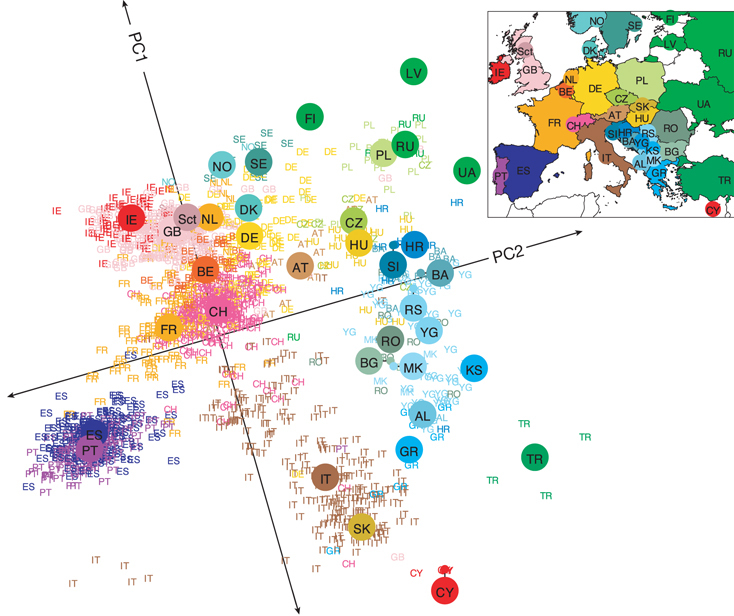
\includegraphics[width=0.62\linewidth]{genetics-pca-europe-map}\hspace{-1cm}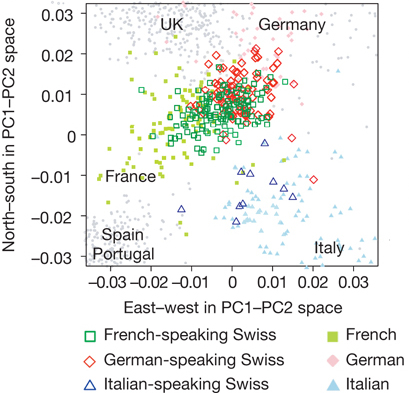
\includegraphics[width=0.32\linewidth]{genetics-pca-europe-swiss}

\vspace{0.5cm}
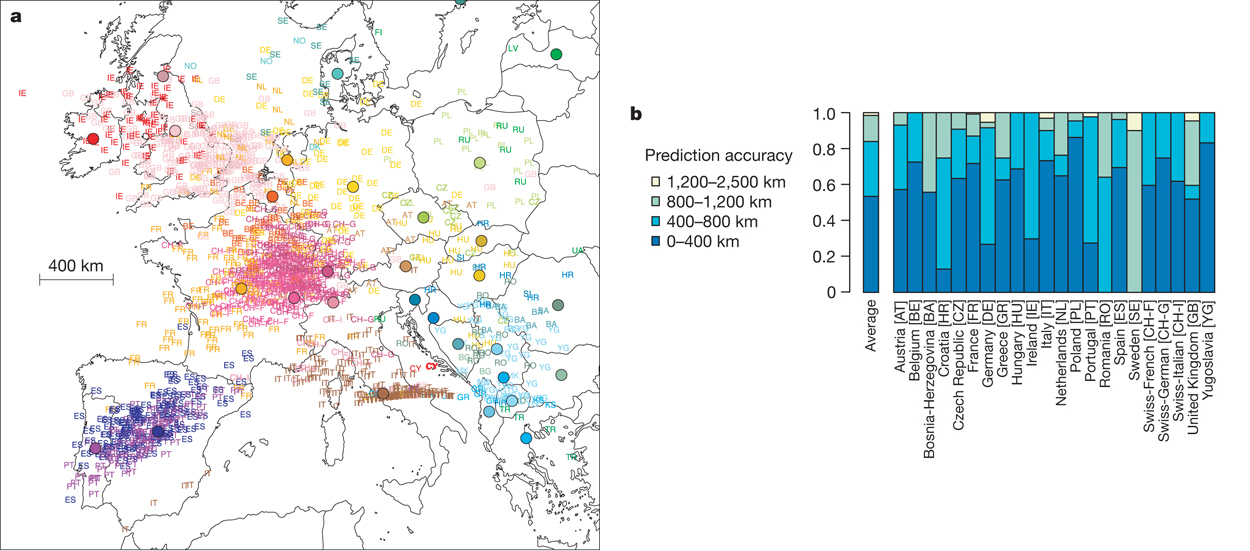
\includegraphics[width=0.75\linewidth]{genetics-pca-europe-cvpred}
\caption{Interspersed goal - Communicating PCA embedding to 2D, cluster identity (from metadata) and geographical matching in the same figure. (top) PCA embedding of genetic sequencing data, in 2D, colored by nationality, cluster center of masses indicated. (top, inset) zoom in on Swiss population, colored by mother-tongue. (bottom) geographical prediction accuracy of sample location, split by country.  }
\end{center}
\end{figure} 

\clearpage

\section{Mathematical concepts}

\textbf{Goal:} Find the manifold.\\

More precisely, find $\mathbf{y}_i \in \mathbb{R}^{D_y} ,\; (D_y < D_x)$ so that $\mathbf{y}_i$ parameterises the location of $\mathbf{x}_i$ on the manifold.

\begin{center}
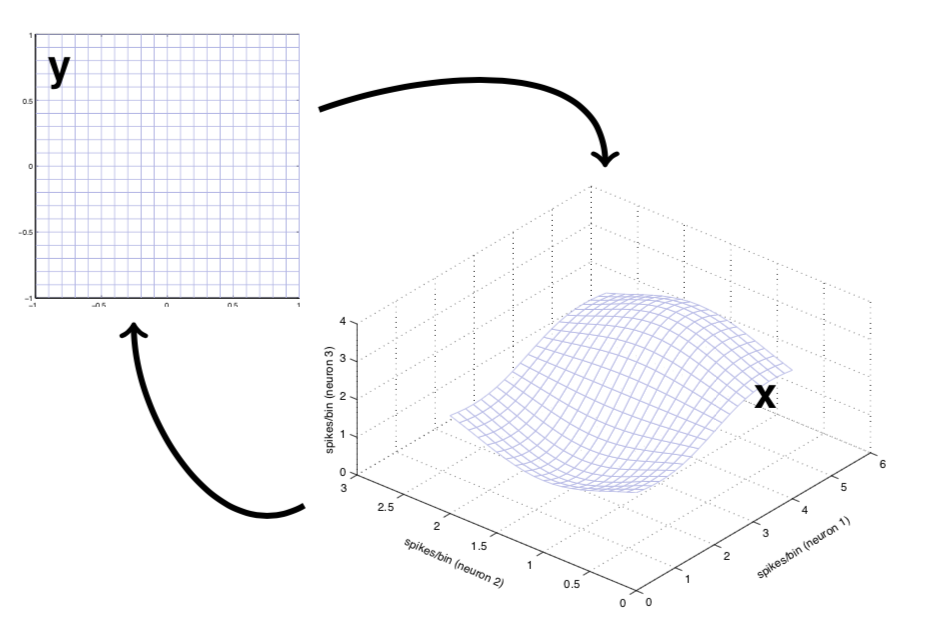
\includegraphics[width=0.7\linewidth]{dimred_manifold_embed}	
\end{center}


\textbf{Core ideas:}
    \begin{itemize}
    \item preserve ``local'' structure
    \item preserve ``information''
    \end{itemize}

\subsection{Linear methods}
(PCA, MDS)
\\

Let $\mathbf{y}_i = P^\top \mathbf{y}_i$ for a projection matrix $P^\top$.\\[1ex]

$P \in \mathbb{R}^{D_x\times D_y}$ defines a linear mapping from data to manifold, and vice versa.  \\[1ex]


Linearity
\begin{itemize}
\item preserves local structure  
\item preserves global structure
\end{itemize}




\subsubsection{PCA - Principal component analysis}

\textbf{Idea:} look for projection that keeps data as spread out as possible
$\Rightarrow$  most variance, means it preserves most "information" \emph{(Knowing the location of a point along a direction where points are more spread out helps us identify the point more!)}

\vspace{0.5cm}

\begin{tcolorbox}[title=PCA algorithm]

PCA directly implements this idea:

\begin{itemize}
	\item Find the direction with the greatest variance.
	\item Project the data onto it (residuals now live in $D_x - 1$ dimensions)
	\item Repeat until a set maximum embedding dimensions, or when residual variance drops below a given threshold
\end{itemize}

\end{tcolorbox}

A collection of data points 

$$\{\ \mathbf{x}_i \in \mathbb{R}^{D_x\times N} \}_{i=1}^N $$

can be represented as a matrix, where each column is a data point

$$ [\ \mathbf{x}_1,\  \mathbf{x}_2,\  \cdots,\  \mathbf{x}_N\ ] = \mathbf{X} \in \mathbb{R}^{D_x\times N}$$

PCA then acts as a matrix factorisation on the "scatter matrix", that is the average of outer products, or the scaled empirical covariance matrix

$$ \mathbf{S} = \frac{1}{N}\sum_{i=1}^N (\mathbf{x}_i - \mathbf{x_{\textrm{mean}}})(\mathbf{x}_i - \mathbf{x_{\textrm{mean}}})^\top = \frac{1}{N} \mathbf{X}_c\mathbf{X}_c^\top $$


 In general, the principal components are exactly the eigenvectors of the empirical covariance matrix $\mathbf{S}$, ordered by decreasing eigenvalue. 
 
 The PCs are the columns of the projection matrix $P$, and they define a $D_y$ dimensional linear manifold. Each $\mathbf{y}_i$ represent a set of coordinates on the low-dimensional manifold.
 
  \clearpage

\begin{tcolorbox}[title=PCA uses \#1]

 We can compute the $\mathbf{y}_i$, the \textbf{"coordinates on the embedded manifold"} via the projection matrix:
 
$$\mathbf{y}_i = P^\top \mathbf{x}_i$$

This emphasizes the use of PCA for the following goals:

\begin{itemize}
	\item Manifold discovery (find and parametrise a low dimensional manifold to project into)
	\item Feature discovery (The discovered PCs - the columns of the $P$ projection matrix) are often meaningful, and may be interpreted.
	\item Visualisation - The high dimensional data may be shown as embedded in low-D, with keeping as much "information" as possible (PCA is the optimal linear method).
\end{itemize}

\begin{center}
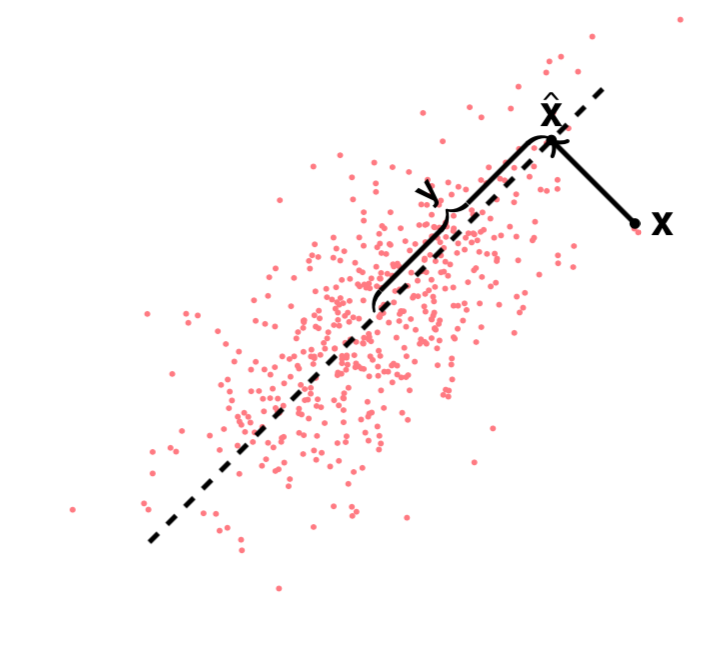
\includegraphics[width=0.75\linewidth]{dimred_pca_project}	
\end{center}


\end{tcolorbox}

\clearpage


\vspace{1cm}

\begin{tcolorbox}[title=PCA uses \#2]

But also we can find a \textbf{"reconstruction"} of the original point via projecting back from the embedding

$$\hat{\mathbf{x}}_i = P \mathbf{y}_i, $$ 

and combining both operations, we can estimate a \textbf{"lossy reconstruction"} of a data point $\mathbf{x}_i$:

$$ \hat{\mathbf{x}}_i = P P^\top \mathbf{x}_i $$

This gives rise a number of interesting views of PCA (and dimensionality reduction in general), as it can be used for

\begin{itemize}
	\item Denoising ($\hat{\mathbf{x}}$ is a less noisy version of $\mathbf{x}$)
	\item Compression (even though we accept $\hat{\mathbf{x}}$ as imperfect, representing only $\mathbf{y}$ and $P$ may take significantly less space, for eg. jpeg format)
	\item Autoencoding is basically the same as denoising, but we assume the embedding and the reconstrucing projections may be different (even though in PCA they are transposes of one-another). \emph{A linear autoencoder neural network trained to minimise squared error learns to perform PCA (Baldi \& Hornik, 1989).}
\end{itemize}


\hspace{2cm}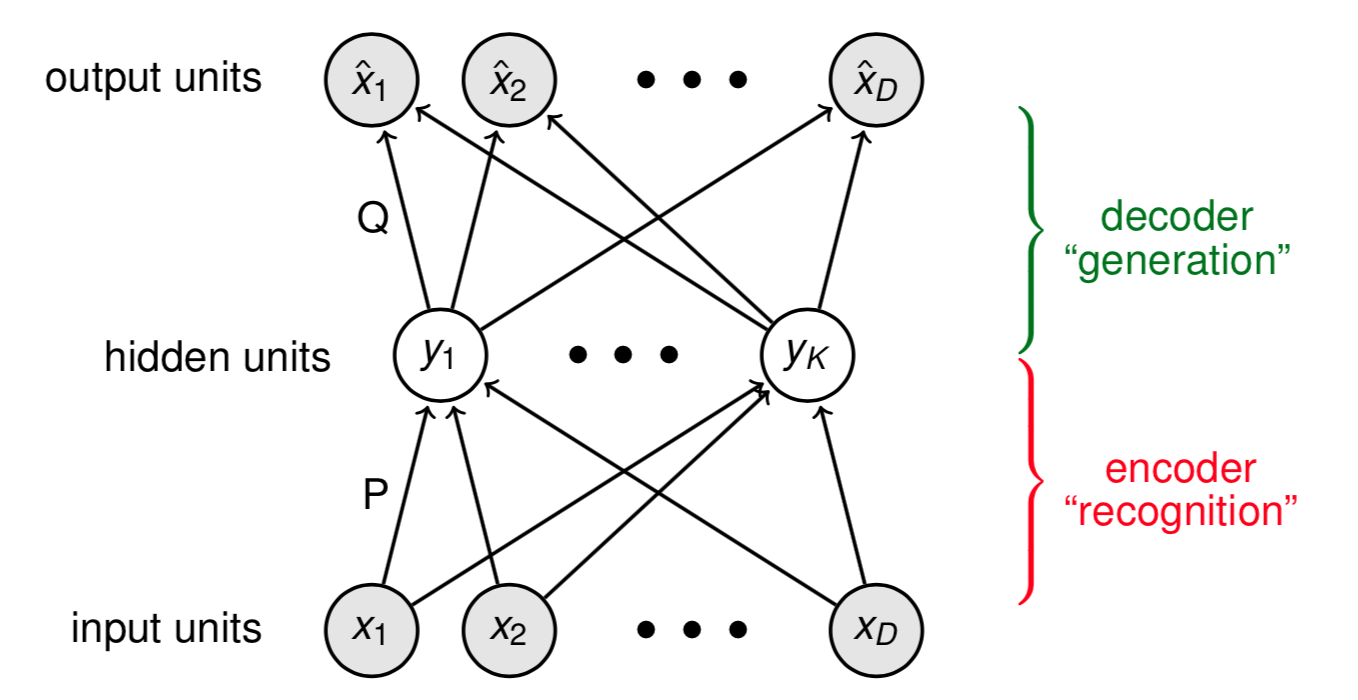
\includegraphics[width=0.8\linewidth]{dimred_pca_autoencode}	
\end{tcolorbox}

\clearpage

There are a number of extensions to PCA, that target different issues:

\begin{itemize}
	\item PCA assumes that noise only affects "out-of-manifold" dimensions, and all dimensions are weighted equally.
	\begin{itemize}
		\item pPCA (probabilistic PCA) assumes that noise is isotropic (affects all dimensions equally), and takes it into account when estimates the signal
		\item FA (factor analysis) allows for independent noise along each dimension
	\end{itemize}
	\item The autoencoder view is only optimal if the projections are linear. Non-linear autoencoders (such as multilayer neural networks) are implementing the same idea - to learn compressed, yet effective representations - much more powerfully.
\end{itemize} 


\subsubsection{MDS - Multidimensional scaling}

Suppose all we were given were distances or symmetric
``dissimilarities'' $\Delta_{ij}$.

\[
\Delta =
\begin{bmatrix}
  0 & \Delta_{12} & \Delta_{13} & \Delta_{14} \\
  \Delta_{12} & 0 & \Delta_{23} & \Delta_{24} \\
  \Delta_{13} & \Delta_{23} & 0 & \Delta_{34} \\
  \Delta_{14} & \Delta_{24} & \Delta_{34} & 0 \\
\end{bmatrix}
\]

\vspace{0.5cm}

\textbf{Goal}: Find vectors $\mathbf{y}_i$ such that $\| \mathbf{y}_i - \mathbf{y}_j
\| \approx \Delta_{ij}$. 

\vspace{0.5cm}

This is called \textbf{Multidimensional Scaling (MDS)}.

\vspace{0.5cm}
Given the some numeric data $\mathbf{X}$, we can compute the Euclidean distances $\Delta_{ij} = \| \mathbf{x}_i - \mathbf{x}_j \| $. The resulting optimal MDS embedding (that now attempts to keep the distances intact, rather than the maximising the variance retained like PCA) is exactly \textbf{equivalent to the PCA embedding!} This is called a \textbf{"dual representation"}.

\begin{tcolorbox}[title=MDS advantages]

Why would then we ever use MDS then?
% Nice summary: https://cseweb.ucsd.edu/~saul/papers/smdr_ssl05.pdf

\vspace{0.5cm}
 
Representing data as purely the pairwise dissimilarities between data points is a very powerful idea:

\begin{itemize}
	\item  (nonmetric MDS) We can work on arbitrary, non-numeric datasets as well, as long as we can somehow compute pairwise dissimilarities (see kernel PCA below). 
	\item (metric graph-based MDS) We can replace the Euclidean distances with other distance calculations, that lead to other algorithms:
	\begin{itemize}
		\item[$\rightarrow$] Isomap uses approximate geodesic distances (distances along an estimated non-linear manifold)
		\item[$\rightarrow$] Maximum Variance Unfolding (MVU) preserves only distances amongst k nearest neighbours%, then maximises variance given those constraints
		\item[$\rightarrow$] Locally linear embedding (LLE) defines non-symmetric distances that represent local linear reconstructability  % preserves local "linear reconstructability" amongst k nearest neighbours (more on this later).
	\end{itemize} 
	\item (kernel PCA) The distance preservation problem can actually be rewritten in a different form, that attempts to minimise the difference in inner products (Gramian matrices) in the original and embedding spaces:
	
	$$ \argmin_{\{\, \mathbf{y}_i\, \}_{i=1}^N} \sum_{i=1}^N\sum_{j=1}^N (\mathbf{x}_i^\top \mathbf{x}_j - \mathbf{y}_i^\top \mathbf{y}_j ) $$
	
	A popular non-linear extension is to replace the inner products $\mathbf{x}_i^\top \mathbf{x}_j$ with a positive definite kernel function $k(\mathbf{x}_i, \mathbf{x}_j)$, and solve for $\mathbf{y}$ vectors that preserve these modified set of inner products. 
	
	\vspace{0.5cm}
	The popular metric kernel choices ( Gaussian or Polynomial ) are often not well suited for dimensionality reduction. The graph-based algorithms can be seen as a special case of kernel PCA with approximate data-dependent graph kernels (that are defined by neighborhood relationships).
	
	\vspace{0.5cm}
	We can also define kernels over non-metric input spaces (such as bag of words for text mining), which lead 
	
	
\end{itemize}

\end{tcolorbox}


\subsection{Non-linear methods}

\subsubsection{Isomap}

\subsubsection{LLE}

\subsubsection{t-SNE}


\section{Application to "Frey Face" dataset}

Interactive python code to gain intuition

\section{Application to scRNA-seq dataset}

Analysis via various dimensionality reduction method and group discussion on results

\section{Dimensionality reduction for DNA microscopy outputs}

TODO


\section{Overview}




%$$ \mathbf{x}_i = \mathbf{X}[:,i] $$







\end{document}
